\section{Module Functions and Integration}
\label{sec:modules}
The architecture in Fig.~\ref{fig:arch} is implemented as cooperating
modules rather than a single monolithic agent. Shared interfaces connect
task execution to configuration, industrial services, protocol drivers, and
route-specific evidence. This section describes those responsibilities and
the checks that preserve their boundaries.

The implementation scope is broader than the evaluated scope. Section~V
separates implemented interfaces from the routes and checks exercised here;
an interface intended for extension does not by itself establish
interchangeability or portability.

The extension contracts expose the data passed at each boundary. A harness
call is normalized as \texttt{HostToolCall(toolName, arguments)} and returns
\texttt{HostToolResult(text, isError)}. A DCW driver accepts an engineering
value, tolerance, range, and driver configuration; its result separates write
status, raw value, readback, and acknowledgment grade (readback-verified,
transport-ack, or unverified). Each DAQ sample stores its node, timestamp,
value, and state, with optional line, product, recipe, and run IDs. A write
anchor records line/node, prior and requested values, source, actor, time, and
optional run/task/approval IDs; recipe definitions retain separate versions.
These fields keep tool errors, device receipts, observations, and production
lineage inspectable as separate records.

DAQ and write-anchor records may omit line, product, recipe, run, task, or
approval identifiers when a route does not supply them. For the R20 trace
audit, the join keys are required: task ID, approval ID, recipe-trial run ID,
active-run ID, and the run ID returned with the sample must agree with the
corresponding route records. R21 checks the corresponding IDs on its
deterministic fixture path. Thus the reported complete joins are requirements
of those evaluated records, not a guarantee that every general record
contains every identifier.

\subsection{Task Runtime and Harness Adapters}
Task and chat access surfaces create or join a workspace channel, where the
task engine manages members, task queues, shared memory, and execution
templates. Direct REST tool calls and selected stdio MCP operation calls can
enter the shared dispatcher without creating a task or invoking a harness;
MCP management and task methods use their corresponding services. A direct
call has no agent-turn prompt context: its operation handler resolves live
route state from request identifiers and service data at invocation.
The harness registry instantiates an adapter behind a common agent interface;
the prompt builder combines the task with the active scene brief, industrial
context, channel profile, agent binding, and retrieved memory. Tool calls
return to the shared dispatcher regardless of which registered harness
produced them. The registry keeps engine-specific execution behind the common
agent interface. Industrial context is assembled for
each agent turn rather than pinned for the task lifetime, so prompt context is
grounding information rather than write authorization. An approved recipe
action separately captures the current line--product--recipe--run tuple when
approval is requested and compares it again before dispatch. This
approval-time check does not imply that the earlier prompt context remained
unchanged.

\subsection{Production Context and Configuration}
Scene blueprints describe devices, signal maps, objectives, and process
guards. A task resolves these definitions against its active
line--product--recipe--run context. The channel profile selects the available
capability family, the tool policy narrows the operation catalog, and the
agent binding scopes the nodes, controls, and recipe operations available to
that member. These filters can restrict one another but cannot broaden the
underlying device range. The dispatcher re-reads policy at execution, so a
cached catalog does not retain authority after a grant or policy change. The
prompt builder assembles the agent's available bound-line and active-run
context on each turn; it does not pin the complete context tuple to the task.
Approved recipe actions capture the active tuple at request time and refuse
dispatch if its line, product, recipe, or run field changes during the
approval wait.
Specific production snapshot, trial, and MPC routes, together with Hybrid Twin
training submissions, resolve and validate a versioned \texttt{SceneContract}
at operation time. The Twin physics-specification draft route can instead
accept a caller-supplied scene description; SceneContract enforcement is
therefore route-specific and does not validate or pin all prompt context.

\subsection{Acquisition, Analysis, and Modeling Services}
Semantic DAQ nodes expose typed values, engineering units, ranges, and
sampling settings while hiding protocol-specific reads. A per-node DAQ
runtime schedules acquisition and stores timestamped observations; the
gateway aggregates node pipelines. MES-facing operations provide the
configured production-data path. Analysis and retrieval services consume
these records, while optional model, training, optimization, and digital-twin
services are invoked through their registered operation handlers. These
services complement the agent workflow; AgentWorkShop does not prescribe a
single optimization strategy.

\subsection{Semantic I/O and Actuation}
The driver registry resolves a semantic node to a built-in or plugin driver.
DAQ handlers use the node's acquisition interface; DCW handlers route a
write or readback through the controller and the configured protocol driver.
This separation lets recipes and agents refer to semantic controls without
embedding Modbus, OPC UA, MQTT, HTTP, or MES transport details in their
operation arguments. The supported driver mappings are implementation
interfaces; only the mappings and workflows enumerated in Section~\ref{sec:eval}
are experimentally exercised.

\subsection{Shared Dispatch and Write Admission}
\label{sec:governed}
Every named operation passes the dispatcher. Its ordered checks validate
invocation scope and current channel policy (tool selection, profile, and
applicable duty separation), then the agent's binding and runtime grant and
ownership of referenced resources.
A refusal returns the excluding condition. Denial persistence is selective:
grant denials and selected resource-reference denials have explicit audit
paths, whereas scope and channel-policy denials are not uniformly retained as
durable audit events. A catalog entry therefore describes availability but
does not authorize execution. Handlers for operations that require manual
approval suspend for a decision, then revalidate authority and active limits
before dispatch. For manual recipe operations, the handler checks the active
run, candidate parameters, and route timing before approval; after the wait it
rechecks current authority and active limits. For \texttt{recipe\_apply}, a
changed definition requires a new proposal. These route-specific checks
complement, but do not replace, the per-call dispatcher checks.

All actuator writes converge on the DCW admission point. For an online node
write, the admissible interval is
\begin{equation}
\mathcal{I}^{\mathrm{online}}_n(t)=\mathcal{H}_n\cap\mathcal{B}_n
\cap\mathcal{P}_n(t)\cap\mathcal{R}_n(t),
\label{eq:admission}
\end{equation}
where $\mathcal{H}_n$ is the hard engineering range and $\mathcal{B}_n$,
$\mathcal{P}_n$, and $\mathcal{R}_n$ are the baseline, active-product, and
active-recipe limits. Missing optional limits impose no restriction, whereas
an empty intersection rejects the request and identifies the excluding
layer. Recipe dispatch applies the hard, baseline, and product limits to the
replacement recipe rather than intersecting with the previous recipe window.
The actuator path also enforces step, interval, and hold-window checks.
These admission rules constrain commands; process objectives and coupled
variable guards are assessed from later observations. The framework does
not replace independent PLC or safety-instrumented protection.

\subsection{Integrated Operation and Route-Specific Evidence}
\label{sec:tasklifecycle}
A recipe trial illustrates how the modules cooperate. The task runtime
delivers a named \texttt{recipe\_trial} call from the agent harness; the
dispatcher checks the agent's recipe binding and execution scope; the recipe
handler checks the active run, candidate parameters, and route timing; and a
manual binding requests approval before the DCW controller sends the batch
through its driver. The handler returns a per-parameter receipt. The caller
then obtains DAQ observations and can request a separate update, apply, or
rollback operation. A trial receipt confirms command handling; it does not
by itself establish process attainment or persist a new recipe version.

The routes retain different records because they answer different
questions. A driver acknowledgment reports command evidence; DAQ reports a
process observation; an exploration summary records a bounded probe; and a
recipe version records a saved definition. Their relation through actor and
production context allows an execution to be inspected without treating
these outcomes as interchangeable.

\subsection{Route-Specific Lifecycles and Evidence}
\label{sec:routes}
\label{sec:mech}
\label{sec:objective}
\label{sec:nodeexec}
\label{sec:ack}

\paragraph{Timing and approval}
Timing guards are route-specific. Online node writes enforce an effective
minimum spacing of 60\,s. Recipe dispatch uses a per-recipe interval anchored
to approval, while trials also use a configurable per-line cadence (default
300\,s). The recipe interval can refuse a proposal before an approval request
is created. Checks occur at proposal or execution according to the operation,
and experiment-specific pacing overrides are reported with the corresponding
results.

Manual bindings create an approval request containing the actor, operation,
candidate values, applicable limits, expiry, parameter bases, and the active
line--product--recipe--run context. The default wait expires after 180\,s and
refuses execution. After approval, the executor rechecks authorization and
compares the current context tuple with the approved tuple. For approved
recipe writes and dispatched rollback, a final synchronous comparison follows
the asynchronous grant check immediately before entering the DCW dispatch
path. Changes visible at this software boundary are refused before a driver
write. This check is not an atomic lock across network or device I/O and
cannot cancel a driver call after it begins. A focused mock-state suite
changes line, product, recipe, or run during approval for recipe apply, trial,
and dispatching rollback; each mutation is refused before a driver write or
new execution record. For
\texttt{recipe\_apply}, a changed recipe definition also requires a new
proposal; an unchanged approval dispatches a copy of the approved parameter
snapshot. A line-level recipe mode defaults to manual; changing it to
automatic requires administrator confirmation. The approval record
authorizes a workflow action and does not replace process protection.

Fig.~\ref{fig:hitl}(a) illustrates the four-layer interval in
Eq.~(\ref{eq:admission}) with an archived RPM configuration; panel (b) shows a
symbolic approval followed by context and authority rechecks. The plotted
values are illustrative and are not R20 measurements.

\begin{figure*}[!t]
\centering
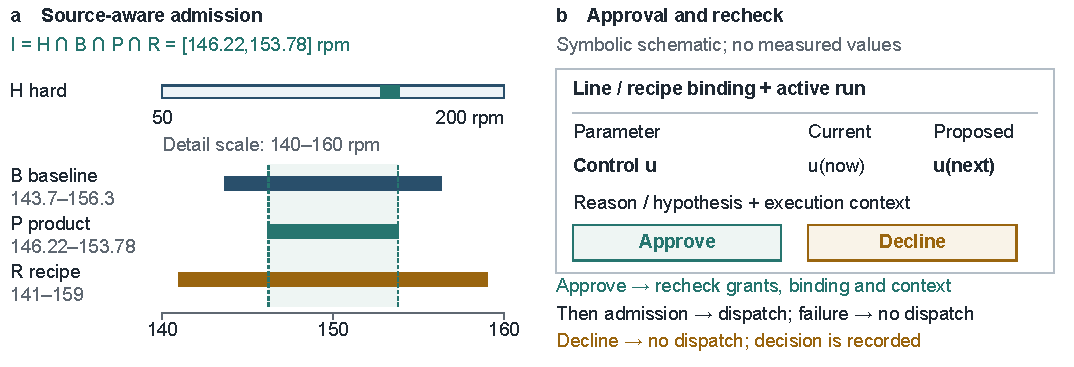
\includegraphics[width=\textwidth]{resources/fig-admission-hitl-2026.pdf}
\caption{Admission and approval boundaries. (a) Illustrative archived RPM
configuration (not part of R20):
online node interventions use the four-layer value interval of
Eq.~(\ref{eq:admission}),
whereas recipe dispatch omits the prior recipe window. (b) Symbolic human
approval binds a proposed action and its context tuple; execution rechecks the
active line--product--recipe--run context, authority, and applicable limits
after approval. Approval does not reserve equipment state.}
\label{fig:hitl}
\end{figure*}

\paragraph{Node probe}
The bounded \texttt{optimization\_explore} route is exposed to the AML
optimization profile. It validates a bound control and DAQ scope, captures a
baseline, routes a bounded write through DCW, and stores a later target window
as a separate exploration summary. Its timing and approval behavior is
route-specific; R20 does not exercise this route.

\paragraph{Recipe operations}
\texttt{recipe\_trial} checks the bound recipe and active run, then dispatches
candidate overrides as a batch with per-parameter verification. The caller
subsequently queries DAQ and may save a definition with
\texttt{recipe\_update}, restore one with \texttt{recipe\_rollback}, or apply
a version with \texttt{recipe\_apply}. A trial does not save or apply a
version, and endpoint verification is not a process-response measurement.
Public direct-node control is closed; bounded probes and recipe operations are
the configured write surfaces.

\paragraph{Command verification}
Command confirmation and process response answer different questions. A
driver ACK is graded as \texttt{readback-verified}, \texttt{transport-ack},
or \texttt{unverified}; a matching endpoint read supports the first grade,
whereas transport or MES application confirmation supports the second.
Recipe-batch verification is \texttt{verified}, \texttt{unverified}, or
\texttt{failed}. If readback is absent or mismatched, up to three reads are
attempted 2\,s apart. Initial ACKs, final ACKs, and per-parameter verdicts are
retained separately. A readback-verified setpoint does not establish target
attainment.

\paragraph{Observation, verdict, and compensation}
Recipe-path observation follows batch dispatch, and saving a definition,
applying it, and observing process response remain separate operations. An
open node record can request rollback after repeated breaches; missing samples
do not count as breaches. Caller verdicts and compensation remain separate
from the observation and subject to admission checks.
\label{sec:agentloop}

